\documentclass[tikz,border=6pt]{standalone}
\usetikzlibrary{arrows.meta}
\definecolor{red}{HTML}{A50F2D}\definecolor{ink}{HTML}{141414}\definecolor{gry}{HTML}{5F5F5F}\definecolor{blu}{HTML}{1F5F99}
\begin{document}
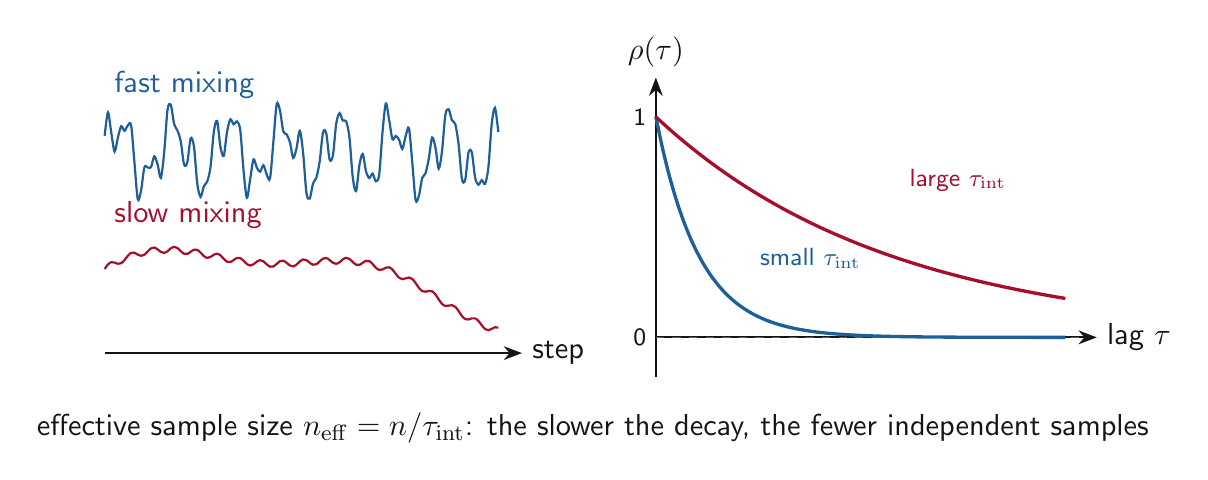
\begin{tikzpicture}[font=\sffamily\fontsize{11}{13}\selectfont,>=Stealth]
% left: two chains
\node[blu,anchor=west] at (0,3.2) {fast mixing};
\draw[blu,thick,smooth,samples=120,domain=0:5] plot (\x,{2.35+0.35*sin(deg(9*\x))+0.25*sin(deg(23*\x+1))+0.15*sin(deg(41*\x))});
\node[red,anchor=west] at (0,1.55) {slow mixing};
\draw[red,thick,smooth,samples=120,domain=0:5] plot (\x,{0.7+0.45*sin(deg(0.9*\x))+0.2*sin(deg(1.9*\x+1))+0.04*sin(deg(23*\x))});
\draw[->,ink,thick] (0,-0.2)--(5.3,-0.2) node[right]{step};
% right: autocorrelation
\begin{scope}[xshift=7.0cm]
\draw[->,ink,thick] (0,0)--(5.6,0) node[right]{lag $\tau$};
\draw[->,ink,thick] (0,-0.5)--(0,3.3) node[above]{$\rho(\tau)$};
\draw[gry,dashed] (0,0)--(5.4,0);
\node[ink,anchor=east,font=\sffamily\small] at (0,2.8) {1};
\node[ink,anchor=east,font=\sffamily\small] at (0,0) {0};
\draw[blu,very thick,smooth,samples=60,domain=0:5.2] plot (\x,{2.8*exp(-\x/0.55)});
\draw[red,very thick,smooth,samples=60,domain=0:5.2] plot (\x,{2.8*exp(-\x/3.0)});
\node[blu,anchor=west,font=\sffamily\small] at (1.2,1.0) {small $\tau_{\mathrm{int}}$};
\node[red,anchor=west,font=\sffamily\small] at (3.1,2.0) {large $\tau_{\mathrm{int}}$};
\end{scope}
\node[ink,align=center,font=\sffamily\fontsize{11}{13}\selectfont] at (6.2,-1.15) {effective sample size $n_{\mathrm{eff}} = n/\tau_{\mathrm{int}}$: the slower the decay, the fewer independent samples};
\end{tikzpicture}
\end{document}
